\newpage
\hypertarget{stringRep vis}{}
\subsection{Implementing stringRep}
\visHeader

\begin{itemize}

\item[$\blacktriangleright$] Go ahead and create the SDM for \texttt{Box::toString} until it closely resembles Fig.~\ref{fig:sdm_tostring_1}. 

\vspace{0.5cm}

\begin{figure}[htbp]
\begin{center}
  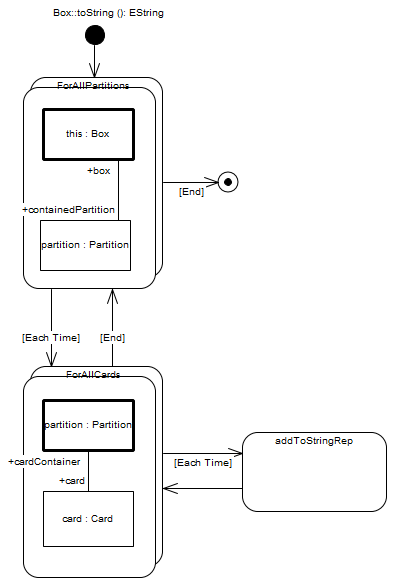
\includegraphics[width=0.8\textwidth]{ea_toStringStart}
  \caption{Control flow with nested loops} 
  \label{fig:sdm_tostring_1}
\end{center}
\end{figure}

\clearpage

\item[$\blacktriangleright$] To briefly discuss the edge guards, whenever a \texttt{For Each} node has multiple activity edges to different nodes, it requires
both an \texttt{Each Time} and \texttt{End}. In the case of \texttt{ForAllPartitions}, we want each iteration to go to \texttt{ForAllCards} and then, once that
is complete, proceed to the stop node. If there were no guards, it could (potentially) immediately proceed to the stop node. Similarly, in \texttt{ForAllCards},
we want the flow to access \texttt{addToStringRep} each time, then return to the partition loop once finished.

\vspace{0.5cm}

\item[$\blacktriangleright$] Now, while \texttt{addToStringRep} has been created, its default story node state will not allow it to access the our helper
method. Double-click the node to invoke its editor and update the \texttt{type} to a \texttt{StatementNode}\define{Statement
Node}(Fig.~\ref{fig:updateStatement}). Statement nodes are used to guarantee execution in the control flow and, while we have invoked methods as part of object
variables, using this strategy lets us represent the action as an activity node.

\vspace{0.5cm}

\item[$\blacktriangleright$] Before closing, switch to the \texttt{Statement} tab (Fig.~\ref{fig:editStatement}) to construct the \texttt{MethodCallExpression}.
We want to access the \texttt{Box} object (\texttt{this}) and its \texttt{addToStringRep} method. Update the \texttt{Parameter Values} to \texttt{card} so we
can pass the object variable \texttt{card} to the method \texttt{addToStringRep} as parameter.

\vspace{0.5cm}

\begin{figure}[htbp]
   \centering
      \subfloat[Update the \texttt{addToStringRep} node]{
        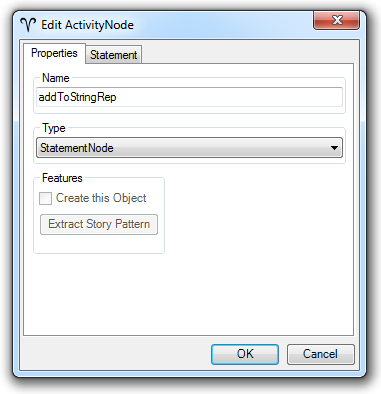
\includegraphics[width=0.5\textwidth]{ea_updateToStatement}
        \label{fig:updateStatement}
      }
      \subfloat[Edit the \texttt{MethodCallExpression} ]{
        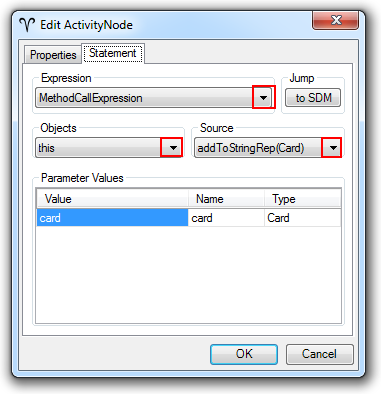
\includegraphics[width=0.5\textwidth]{ea_editStatementNode}
        \label{fig:editStatement}
      }
      \caption{}
\end{figure}
\FloatBarrier

\end{itemize}

Statement nodes should be used to interact with methods that are implemented by hand as they provide a means of invoking libraries and arbitrary Java code from
SDMs. Please note that we do not differentiate at this point between methods that are implemented via an SDM or by hand and thus, statement nodes can of course
be used to invoke other SDMs via a MethodCallExpression. Most importantly, this enables \emph{recursion} as the current SDM can be invoked on \texttt{this} with
appropriate new arguments.

A final point to note is that the return value of methods called from statemend nodes are ignored. These are therefore best used for void methods that
manipulate their arguments (or other appropriate side effects). We shall learn in a few pages how to invoke methods with non-primitive return values (if a
method returns a primitive then it can be invoked in an attribute constraint as in \hyperlink{sec:growBox}{Sec. 5}).

\begin{itemize}

\item[$\blacktriangleright$] Therefore, to complete the SDM, return the final string representation value of the box via an \texttt{AttributeValueExpression} in
the stop node (Fig.~\ref{fig:toStringStopNode}).

\begin{figure}[htbp]
\begin{center}
  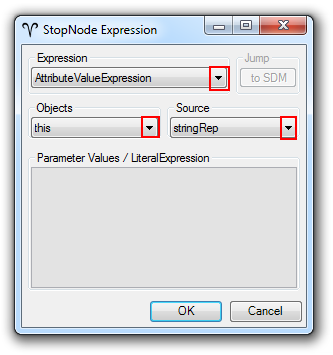
\includegraphics[width=0.5\textwidth]{ea_returnAttributeStopNode}
  \caption{Specify a return value}
  \label{fig:toStringStopNode}
\end{center}
\end{figure}

\item[$\blacktriangleright$] Take some time to compare and reflect on the complete SDM as depicted in Fig.~\ref{fig:sdm_tostring_5}.  The idea was to abstract
from the actual text representation of the box and model the necessary traversal of the data structure. The helper methods \texttt{addToStringRep} could, for example, build up a
string buffer and update this string representation. While modelling this SDM, we have seen that \emph{for each} stroy nodes can be nested, and have learnt two
new uses of MethodCallExpressions that provide a type safe\footnote{Apart from the literal expressions used for specifying argument values} means of invoking
methods from SDMs.

\begin{figure}[htbp]
\begin{center}
  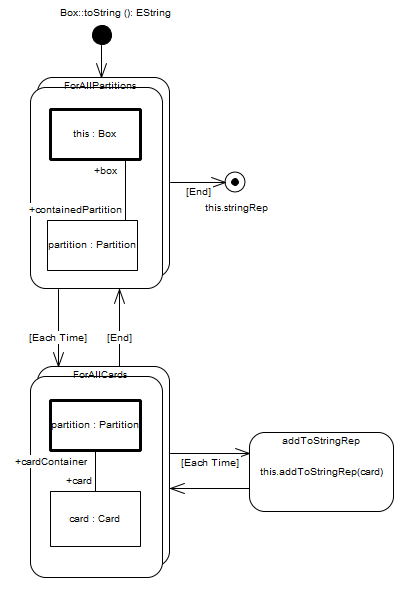
\includegraphics[width=0.8\textwidth]{ea_toStringComplete}
  \caption{The complete SDM for \texttt{Box::toString}}  
  \label{fig:sdm_tostring_5}
\end{center}
\end{figure}
\FloatBarrier

\item[$\blacktriangleright$] You know the drill -- save, validate, and build in Eclipse. To see how this is done in the textual syntax, check out the nested
loops in Fig.~\ref{fig:toStringFlow} and each pattern in Fig.~\ref{fig:toStringPatterns}

\jumpSingle{sec:fastCard}

\end{itemize}
